\documentclass[12pt]{article}
\usepackage{hyperref}
\usepackage{graphicx}
\usepackage[font=small,labelfont=bf]{caption}
\title{Analisi sito}
\date{}
\author{carlo Sindico}
\begin{document}
\pagenumbering{arabic}



\begin{titlepage}

\newcommand{\HRule}{\rule{\linewidth}{0.5mm}} % Defines a new command for the horizontal lines, change thickness here

\center % Center everything on the page
 
%----------------------------------------------------------------------------------------
%	HEADING SECTIONS
%----------------------------------------------------------------------------------------

\textsc{\LARGE Universit\`a degli Studi di Padova}\\[1.5cm] % Name of your university/college
\textsc{\Large Laurea in Informatica}\\[0.5cm] % Major heading such as course name
\textsc{\large Corso di Tecnologie Web 2}\\[0.5cm] % Minor heading such as course title

%----------------------------------------------------------------------------------------
%	TITLE SECTION
%----------------------------------------------------------------------------------------

\HRule \\[0.4cm]
{ \huge  Progetto di fine corso}\\[0.3cm] % Title of your document
\HRule \\[1.5cm]
 
%----------------------------------------------------------------------------------------
%	AUTHOR SECTION
%----------------------------------------------------------------------------------------

\begin{minipage}{0.4\textwidth}
\begin{flushleft} \large
\emph{Studente:}\\
Carlo \textsc{Sindico} % Your name
\end{flushleft}
\end{minipage}
~
\begin{minipage}{0.4\textwidth}
\begin{flushright} \large
\emph{Matricola:} \\
\textsc{1069322} % Supervisor's Name
\end{flushright}
\end{minipage}\\[4cm]

% If you don't want a supervisor, uncomment the two lines below and remove the section above
%\Large \emph{Author:}\\
%John \textsc{Smith}\\[3cm] % Your name

%----------------------------------------------------------------------------------------
%	DATE SECTION
%----------------------------------------------------------------------------------------

{\large 12/06/2016}\\[3cm] % Date, change the \today to a set date if you want to be precise

%----------------------------------------------------------------------------------------
%	LOGO SECTION
%----------------------------------------------------------------------------------------

%\includegraphics{Logo}\\[1cm] % Include a department/university logo - this will require the graphicx package
 
%----------------------------------------------------------------------------------------

\vfill % Fill the rest of the page with whitespace

\end{titlepage}
\newpage
\renewcommand{\contentsname}{Indice}
\tableofcontents

\newpage
\pagenumbering{arabic}

\section{Una breve introduzione}
\subsection{Liceo Leopardi Majorana}
\begin{itemize}
	\item Il sito fornisce uno spazio web per le scuole superiori Liceo Leopardi Majorana. Il sito \'e\ destinatinato a diverse categorie di persone:
	\item per tutte le persone che sono interessate a visitare la scuola, il sito offre una sezione apposita,su come raggiungere la scuola, e anche la storia del liceo.
	\item gli studenti hanno la possibilit\'a\ di visualizzare i propri voti e la media scolastica(accedendo al registro elettronico) e di accedere ad una piattaforma moodle, a cui possono iscriversi,dove sono presenti tutti gli insegnamenti; oltre a visualizzare le news su attivit\'a\ o progetti che la scuola organizza.il sito offre agli studenti una sezione dedicata alla biblioteca presente all'interno della scuola, con un opportuno catalogo (anche se in una versione minimale) dei libri presenti in essa. altre funzionalità offerte agli studenti sono la visualizzazione del calendario e degli orari delle lezioni.
	\item gli insegnanti hanno la possibilit\'a\ di accedere a diverse sezioni d sito come le graduatorie di istituito(gli insegnanti visualizzano quali classi gli sono state assegnate). gli insegnanti inoltre gestiscono il registro elettronico.
\end{itemize}

\subsection{Guida basilare al sito}
La pagina principale \'e\ accessibile dall'indirizzo  \url{http://www.leomajor.gov.it/},ad un primo impatto chi visita il sito,visualizza le news e ultime notizie relative a progetti
o attivit\'a\ che si sono svolte durante l'anno. Il menu principale invece evidenzia le sezioni alle quali l'utente pu\'o\ accedere come ad esempio il registro elettronico(per conoscere i voti), gli orari e il calendario delle lezioni.(le principali).
\textbf{N.B. Questa analisi di usabilit\`a \`e stata redatta nel periodo di fine maggio / inizio giugno 2016, eventuali contenuti del sito potrebbero essere cambiati nel tempo.}


\newpage
\section{Analisi di usabilit\'a\ della homepage}
\subsection{A prima vista}
Per prima cosa cercheremo di analizzare la pagina principale tramite gli occhi di un utente che visita il sito per la prima volta: riesce a capire dove si trova?, e quello che cerca?. Vediamo se le 6W vengono soddisfatte.

\begin{figure}[ht!]
\centering
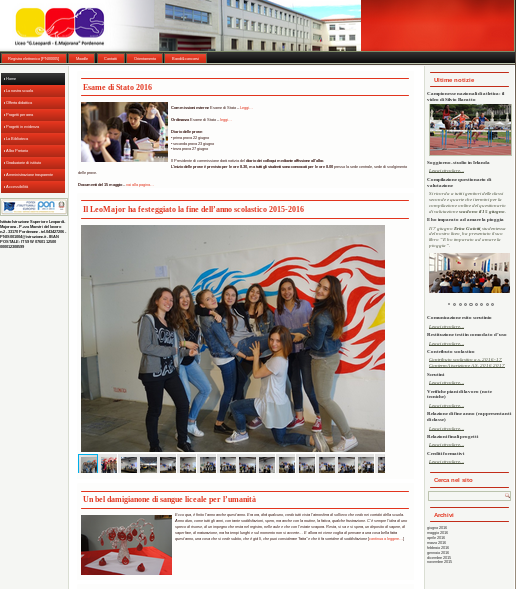
\includegraphics[width=90mm]{home}
\caption{vedi file home.png}
\end{figure} 


\subsubsection{What} Cosa trovo in questo sito?
\begin{itemize}
	\item Sembra un p\'o\ di tutto i contenuti non sono correlati tra loro, si parla di news, eventi progetti, gite scolastiche. Non vi sono categorie che permettano di suddividere l'informazione. un Mix che pu\'o\ confondere l'utente.(disorientamento) Quindi l'utente ad un primo impatto potrebbe non trovare subito l'informazione che cercava; inoltre la barra di ricerca non è presente in alto a destra quindi non subito visibile all'utente,(si deve fare dello scroll per cercarla, e questo implica frustazione)(l'asse where ne parleremo alla successiva sezione..)
\end{itemize}
\subsubsection{Who} Chi c'\'e\ dietro questo sito?
\begin{itemize}
	\item Possiamo notare che il logo \`e\ in alto a destra, ben visibile e con un nome che lo identifica. Sotto questo aspetto l'utente capisce subito che si tratta di  un sito che identifica una scuola.
\end{itemize}
\subsubsection{Where} Dove ci troviamo?
\begin{itemize}
	\item Si pu\`o\ subito notare che vi sono pochi strumenti che offrono all'utente la possibilit\`a di orientarsi:
	l'assenza di qualsiasi tipo di breadcrumb(attributo,path), non permette all'utente
	di sapere dove si trova.Soprattutto per le pagine che riguardano le news. Molto spesso il motore di ricerca per fornire all'utente il risultato pi\`u\ ra pidamente possibile, catapulta l'utente in una pagina interna e non nella homepage. quindi bisogna considerare tutte le pagine interne come delle homepage.
	L'unico strumento che aiuta l'utente \`e l'evidenziazione in nero del menu in corrispondenza della pagina in cui ci troviamo.
	Quando l'utente inizia ad esplorare le pagine interne in particolare le news, non viene salvato il percorso che ha fatto, e quindi \`e\ pi\`u\ proprenso a cliccare il pulsante back.
\end{itemize}
In conclusione, l'utente medio \`e inizialmente spaesato e pi\`u propenso ad abbandonare il sito che a restarci, ma se continua ad esplorarlo capisce man mano il suo funzionamento.

\begin{figure}[ht!]
\centering
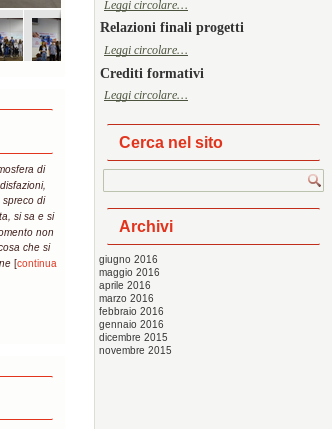
\includegraphics[width=90mm]{search}
\caption{vedi file search.png}
\end{figure} 

\subsubsection{Why} Perch\`e dovrei cercare le informazioni che mi interessano sul sito Liceo Leopardi Majorana e non altrove?. Per coloro che vogliono iscriversi ad una scuola come il Liceo, il sito offre numerose informazioni:
ad esempio dove si trova la scuola, in particolare se il liceo comprende pi\`u sedi oppure un unica sede; i corsi e le materie che gli studenti dovranno frequentare..e tanto altro materiale che pu\`o essere utile per chi vuole affrontare un nuovo percorso di studi al Liceo.

\begin{figure}[ht!]
\centering
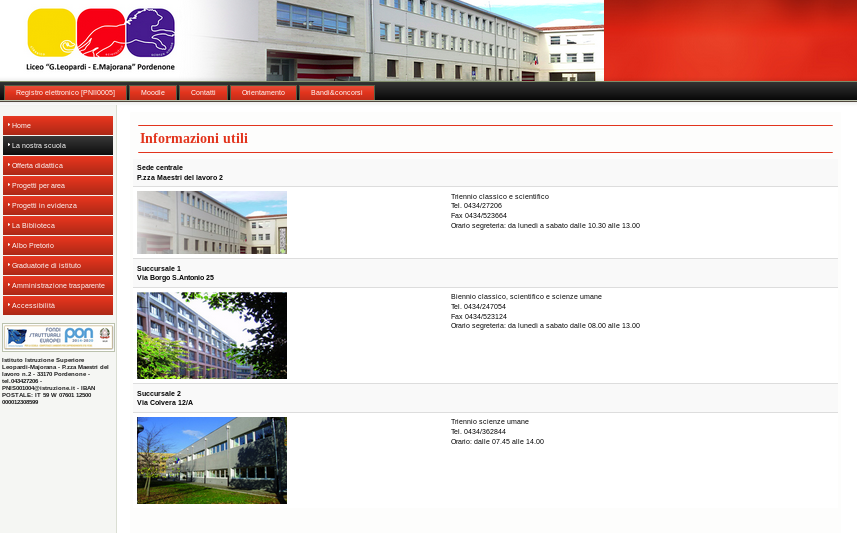
\includegraphics[width=90mm]{informazioniscuola}
\caption{vedi file informazioniscuola.png}
\end{figure} 


\subsubsection{How} Come navigo nel sito?
A questa domanda in parte abbiamo risposto nell'asse where.
Sono presenti pochi strumenti di navigazione, tralasciando il menu a tendina, la barra di ricerca non si trova in una posizione standard (in basso a destra a met\`a pagina) permette all'utente di cercare le infromazioni che gli interessando, ma la posizione ne compromette l'usabilit\`a.

\subsubsection{When} Quali sono le novit\`a del sito?
Come abbiamo accennato prima il sito si incentra sulla pubblicizzazione di news, progetti e attivit\`a che si sono svolte al Liceo, per questo motivo si pu\`o notare che il contenuto della homeage \`e dinamico, tutto il contenuto dinamico ricopre il layout, proprio per mettere in risalto il contenuto stesso. Da notare l'assenza di pubblicit\`a (vedi paragrafo pubblicit\`a).


\subsection{Altri elementi nella pagina}
Il sito adotta una semplice struttura a pannelli: un pannello superiore (header), tre pannelli, di cui due laterali (uno dedicato al men\`u di navigazione a l'altro alle news) e un pannello inferiore (footer).  il sotto-pannello centrale che funge da "nav" \`e situato a sinistra, mentre il contenuto si trova sul pannello centrale e anche sul pannello laterale.
 Questa scelta strutturale fa in modo che l'attenzione dell'utente (che ricordiamo effettua una scansione della pagina ad "F" prediligendo ovvero il lato sinistro dello schermo) sia da subito rivolta al menu di navigazione in questo modo per\`o non si predilige il contenuto della pagina e quindi si accorciano anche se in modo non significativo i timer di permanenza dell'utente nel sito.

\subsection{Pubblicit\`a}
In tutte le pagine del sito non \`e presenete alcun banner pubblicitario, ne popup e questa risulta essere molto positivo per quanto riguarda l'usabilit\`a del sito in quanto aumenta il timer di permanenza dell'utente.

\newpage
\section{Analisi contenuto}
\subsection{Contenuto nella Homepage}
\begin{itemize}
	\item Ne abbiamo gi\`a accenato prima sul fatto che la homepage sia ricca di contenuto che si basa su news progetti e attivit\`a svolte all'interno della scuola. Ora faremo un'analisi pi\`u' dettagliata:
	Possiamo notare come il contenuto nella homepage sia prevalentemente immagini oppure slider di immagini, il contenuto testuale \`e relativo solamente alle immagini. il contenuto testuale \`e  molto spaziato e separato, questo porta ad uno scanning pi\`u  veloce da parte dell'utente. Inoltre si pu\`o  notare come i paragrafi siano strutturati:
	non viene descritto l'intera informazione ma solo una parte e si ai lettori interessati un link. in questo modo si aumenta il timer dell'utente.	 
\end{itemize}
\subsection{Contenuto nelle pagine interne}

	  Il contenuto di alcune pagine interne risulta pi\`u compatto, non vi sono sottoparagrafi, solo qualche piccola lista. La grande quantit\`a di testo rende quindi abbastanza difficile la lettura, dovuta anche al fatto che il font risulta essere piccolo rispetto alle dimensioni consigliate.(da rivedere).
	in generale nella maggior parte delle pagine del sito il contenuto \`e scarno e si rimanda alla lettura completa attraverso link, questo \`e positivo come abbiamo ribadito in precedenza.


\newpage
\section{Considerazioni generali}
\begin{itemize}
	\item Il template adottato da ogni pagina ricalca quello a pannelli della pagina principale, l'unica cosa che cambia \`e parte del contenuto che ovviamente varia a seconda di quello che si vuole motrare. Per i sei assi dell'informazione valgono quindi le stesse cnsiderazioni fatte sulla home.
	Si pu\`o notare che in quasi tutte le pagine,  nella colonna a destra vengono sempre mostrare le news della scuola, e una sezione dedicata all'archivio delle informazioni organizzate per data di inserimento.
	Quindi oltre alla barra di ricerca di cui abbiamo parlato nell'asse where (vantaggi e svantaggi) \`e accompagnata da un archivio con il quale l'utente pu\`o orientarsi meglio.

	Il modo in cui sono suddivide le informazioni e di come reperirle possiamo confermare \`e uno degli aspetti positivi del sito, infatti l'utente quando entra per la prima volta nel sito pu\`o rimanere in un primo tempo spiazzato perch\`e non sa come trovare l'informazione,(barra di ricerca in fondo al sito), ma poi quando si \`e orientato
	pu\`o facilmente reperire ci\`o che gli serviva.

\end{itemize}

\section{Giudizio finale}
In conclusione il sito del Liceo Leopardi majorana non ha di per s\`e molte funzionalit\`a, (a parte la pagina moodle di cui ho preferito tralasciare l'analisi), oltre al solo aspetto informativo, manca un sistema di interazione tra studenti e docenti ad esempio; ma per quanto riguarda il contenuto, le informazioni sono ben visibili, con una buona organizzazione. In base a tutti i punti esaminati durante questa analisi di usabilit\`a assegno a questo sito \textbf{7.5 punti su 10}.

\end{document}
